\section{Route Designer Web Page}
\label{sec:sprint2-web}

For this sprint, the web page described in \autoref{sec:sprint1-web} should be extended with additional functionality to handle friend lists and requests, as well as server side validation of route data. Additionally, users should have access to an elevation profile of their routes.

\subsection{User Interface Changes}
Only one extra view was planned for this sprint; a friend view, only available to users who are already logged in. This view contains three elements:

\begin{itemize}
	\item{A list of the users current friends.}
	\item{A list of incoming friend requests for the user.}
	\item{A form to request friendship from other users.}
\end{itemize}

The friend list should be a simple list of usernames, with the option to remove friends from the list. The request list will also be a list of usernames, but with options whether to accept or deny the request. In this version, the form will simply be a text input field and a submit button, requiring the user to match the desired friend's username exactly. While this is certainly not a perfect solution, it serves the purpose of adding some baseline social functionality to the system.

Additionally, a simple elevation profile of the current route should be added to the route planner view.

Apart from the new elements in the interface, the look of the web page should be overhauled, so that features implemented in the first sprint are more pleasant to use.

\subsection{Database Model Changes}
The database had to be updated to allow for the social aspects. This was accomplished by adding a new table for friends, as can be seen in \autoref{fig:sprint2-db-model}. The \texttt{Friend} table is used to represent both friend requests and established friend relationships, using the \texttt{accepted} column to determine which of the two it is. Apart from this change, the database model is the same as before.

\begin{figure}[!ht]
	\centering
	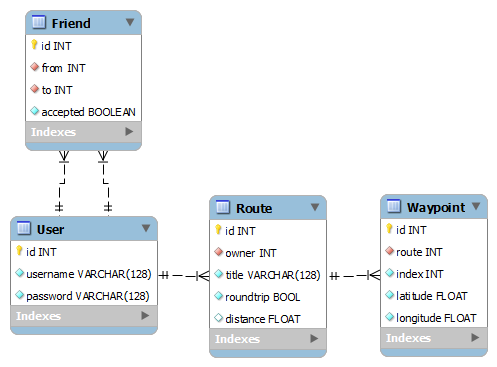
\includegraphics[scale=0.5]{img/sprint2db.png}
	\caption{Sprint 2 Database Model}
	\label{fig:sprint2-db-model}
\end{figure}

\subsection{Implementation}
Once again, the web server development was split into a client part and a server part.

\subsubsection{Server Implementation}
On the server, two separate parts were implemented: The route validation as well as the social systems.

\begin{itemize}
	\item{The route validation consisted mostly of writing a server side version of much of the route planner code, employing the web version of the Google Maps \ac{API}, rather than the javascript version. This means that given a set waypoints, it is possible for the server to construct a version of the route and calculate its distance, just like the client can. Having the distance calculated and stored on the server, has several advantages:}
	\begin{itemize}
		\item{A user cannot send forged data to the server, for example create a route that is 5 kilometres, tell the server it is 10 and use that to get matched up against opponents running harder routes.}
		\item{The server can send the length of each route to the phone application, so presenting the routes to the user does not require recalculating each route on the phone.}
		\item{At some point, the matching system will want access to all of the details of a route, so it can calculate a users progress during a run.}
	\end{itemize}
	Even though the information calculated about a route on the server is considered the correct information, the route designer still presents the information calculated by the client, as this allows for faster information updates during route design.
	\item{The social system was a pretty simple implementation. It provides four different actions:}
	\begin{itemize}
		\item{Sending a friend request to another user. This requires the target user to not already have a friend relationship with the requester (either accepted or pending).}
		\item{Accept and deny incoming friend requests.}
		\item{Remove established friends.}
		\item{Retrieve a list of friends and requests.}
	\end{itemize}
	The main challenge of this was having the server consider entries in the \texttt{Friend} table equal regardless of which user is the \texttt{to} and \texttt{from} user after the request has been accepted, but different while still pending. That is, an accepted friend request makes users mutual friends, while a pending friend request require action from a specific user. This was solved by creating a Django view that retrieves all of a users accepted friends, which can be seen in \autoref{lst:sprint2-get-friends}, while retrieving pending requests was done by filtering requests where the involved user is the \texttt{to} user, as well as \texttt{accepted} set to false.
\end{itemize}

\begin{code}[label={lst:sprint2-get-friends}, caption={'Friend List' function}, language={Python}]
@login_required
def friendlist(request):
	''' Create two lists of Friend instances, inbound and outbound '''
	friends_inbound = Friend.objects.filter(accepted = True, to_user = request.user)
	friends_outbound = Friend.objects.filter(accepted = True, from_user = request.user)
	
	''' Create a list of all users from the "other end" of the inbound request" '''
	friends = [x.from_user for x in friends_inbound]
	''' Extend the list with the "other end" of outbound request. '''
	friends.extend([y.to_user for y in friends_outbound])
	
	return render(request,
	              'friends.html',
	              {'friends': friends,
				   'invites': Friend.objects.filter(to_user = request.user, accepted = False)})
\end{code}

\subsubsection{Client Implementation}
The introduction of elevation profiles was the major point of implementation on the client. Using the Google Maps \ac{API}, getting said elevation profile is very simple. It provides an \texttt{ElevationService} class, which, provided a path in the same format as the one required by the directions service, will return a list of elevation values. These values are then added to a graph using a library called ChartJS\cite{chartjs}, which is presented to the user. This can be seen in \autoref{fig:sprint2-web-screen}, along with the changes made to the \ac{GUI} of the site.

\begin{figure}[!ht]
	\centering
	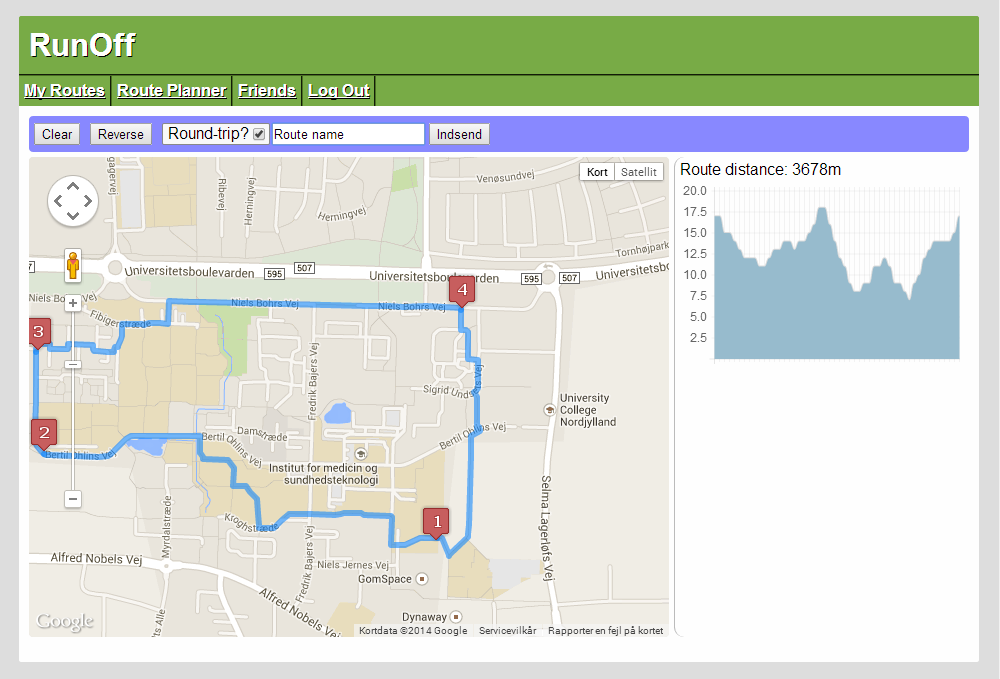
\includegraphics[width=\textwidth]{img/webplanner2.png}
	\caption{Sprint 2 Webpage}
	\label{fig:sprint2-web-screen}
\end{figure}

\subsection{Testing}
Like before, unit testing was done with QUnit and coverage metrics was delivered by Blanket. Code coverage after this sprint was reported to be 82 \%.

Specific unit tests for the server was not written for the server, instead this was tested by making sure the results for each route was the same as those the client calculated. While not extensive, this was deemed to be enough, seeing as the validation is mostly the same calculations that already happened on the client.
